%!TEX root = ../insDoc.tex

\newpage
\section{Numerical Results} \label{sec:numerical_results}

% -------------------------------------------------------------------
\subsection{Manufactured solutions}

\mni
The Matlab code \texttt{runGridConvergence.m} can be used to run grid convergence tests and create a LaTeX table. Before considering exact solutions of Incompressible Navier Stokes flow, we can consider manufacturing solutions of the form
\begin{subequations} \label{eq:TrigMSsolution}
	\begin{align}
		u &= k_y \alpha \cos ( k_x x ) \cos( k_y y) \cos(k_t t) \\
		v &= k_x \alpha \sin ( k_x x ) \sin( k_y y) \cos(k_t t) \\
		p &= \cos (k_x x ) \sin (k_y y) \cos(k_t t)
	\end{align}
\end{subequations}
Where $\alpha$ is some initial velocity amplitude. Note that despite requiring nuanced forcing functions to have these equations satisfy INS, solutions of this form are divergence free and pressure is harmonic.


Here is an example of the convergence rates for our three different time-stepping schemes , (for the implicit method we specify the $\dt$ to use on the coarsest grid, and this is halved each resolution)
\begin{table}[h!]
\footnotesize
\begin{center}

\begin{Verbatim}[fontsize=\small]
runGridConvergence -ts=ab2 -tf=.25 -ms=trig -numResolutions=4 -bcs=pppp
\end{Verbatim}

\input tables/insTSab2BCppppMapCartesianMStrig.tex

\vspace{2em}

\begin{Verbatim}[fontsize=\small]
runGridConvergence -ts=pc2 -tf=.25 -ms=trig -numResolutions=4 -bcs=pppp
\end{Verbatim}
\input tables/insTSpc2BCppppMapCartesianMStrig.tex

\vspace{2em}

\begin{Verbatim}[fontsize=\small]
runGridConvergence -ts=im2 -tf=.25 -ms=trig -numResolutions=3 -bcs=pppp -dtMax=.01
\end{Verbatim}
\input tables/insTSim2BCppppMapCartesianMStrig.tex
\end{center}
\end{table}

\newpage

We can also test the manufactured solutions against different configurations of boundary conditions to see that they are in working order as well:

\begin{table}[h!]
\footnotesize
\begin{center}

\begin{Verbatim}[fontsize=\small]
runGridConvergence -ts=pc2 -tf=.25 -ms=trig -numResolutions=4 -bcs=nnnn
\end{Verbatim}

\input tables/insTSpc2BCnnnnMapCartesianMStrig.tex

\vspace{2em}

\begin{Verbatim}[fontsize=\small]
runGridConvergence -ts=pc2 -tf=.25 -ms=trig -numResolutions=4 -bcs=ssss
\end{Verbatim}
\input tables/insTSpc2BCssssMapCartesianMStrig.tex

\vspace{2em}

\begin{Verbatim}[fontsize=\small]
runGridConvergence -ts=pc2 -tf=.25 -ms=trig -numResolutions=4 -bcs=IIII
\end{Verbatim}
\input tables/insTSpc2BCIIIIMapCartesianMStrig.tex
\end{center}
\end{table}



% ------------------------------------------------------------------------------------
\clearpage
\subsection{Poiseuille Flow} \label{sec:poiseuille_flow}

Consider a fluid in Plane Poiseuille Flow over $[0, 1]^2$ between two no-slip walls at $y = 0$ and $y = 1$ going from pressure $p_{\text{in}}$ to $p_{\text{out}}$ with $p_{\text{in}} > p_{\text{out}}$.
We would define this flow by the following boundary conditions: 
\begin{subequations} \label{eq:PoiseuilleBCs}
	\begin{align}
		\textbf u (x, 0, t) = \textbf u (x, 1, t) = 0 \\
		p(0, y, t) = p_{\text{in}}, \qquad v(0, y, t) \equiv 0 \\
		p(1, y, t) = p_{\text{out}}, \qquad v(0, y, t) \equiv 0 
	\end{align}
\end{subequations}
The fluid then obeys a steady parabolic profile along the flow direction given by
\begin{subequations} \label{eq:Poiseuille}
	\begin{align}
		u &= U(y) = \frac{ p_{\text{in}} - p_{\text{out}} }{ 2 \mu } y (1 - y) \\
		v &\equiv 0 \\
		p &= (p_{\text{out}} - p_{\text{in}}) x + p_{\text{in}}
	\end{align}
\end{subequations}
While we can define the Poiseuille flow as an exact solution for the code to follow, we can also see that defining the initial conditions and appropriate boundary conditions, we are able to get the desired solution to. We can do so in the code by specifying
\begin{Verbatim}[fontsize=\small]
ins -ts=pc2 -tf=10 -N0=40 -nu=0.1
  -ic=zero -bcs=Ionn
  -pressureInflowValue=0 -uInflow=0 -outflowPressureCoeffp=1 -outflowPressureCoeffpn=0 -pOutflow=-1;
\end{Verbatim}
\center
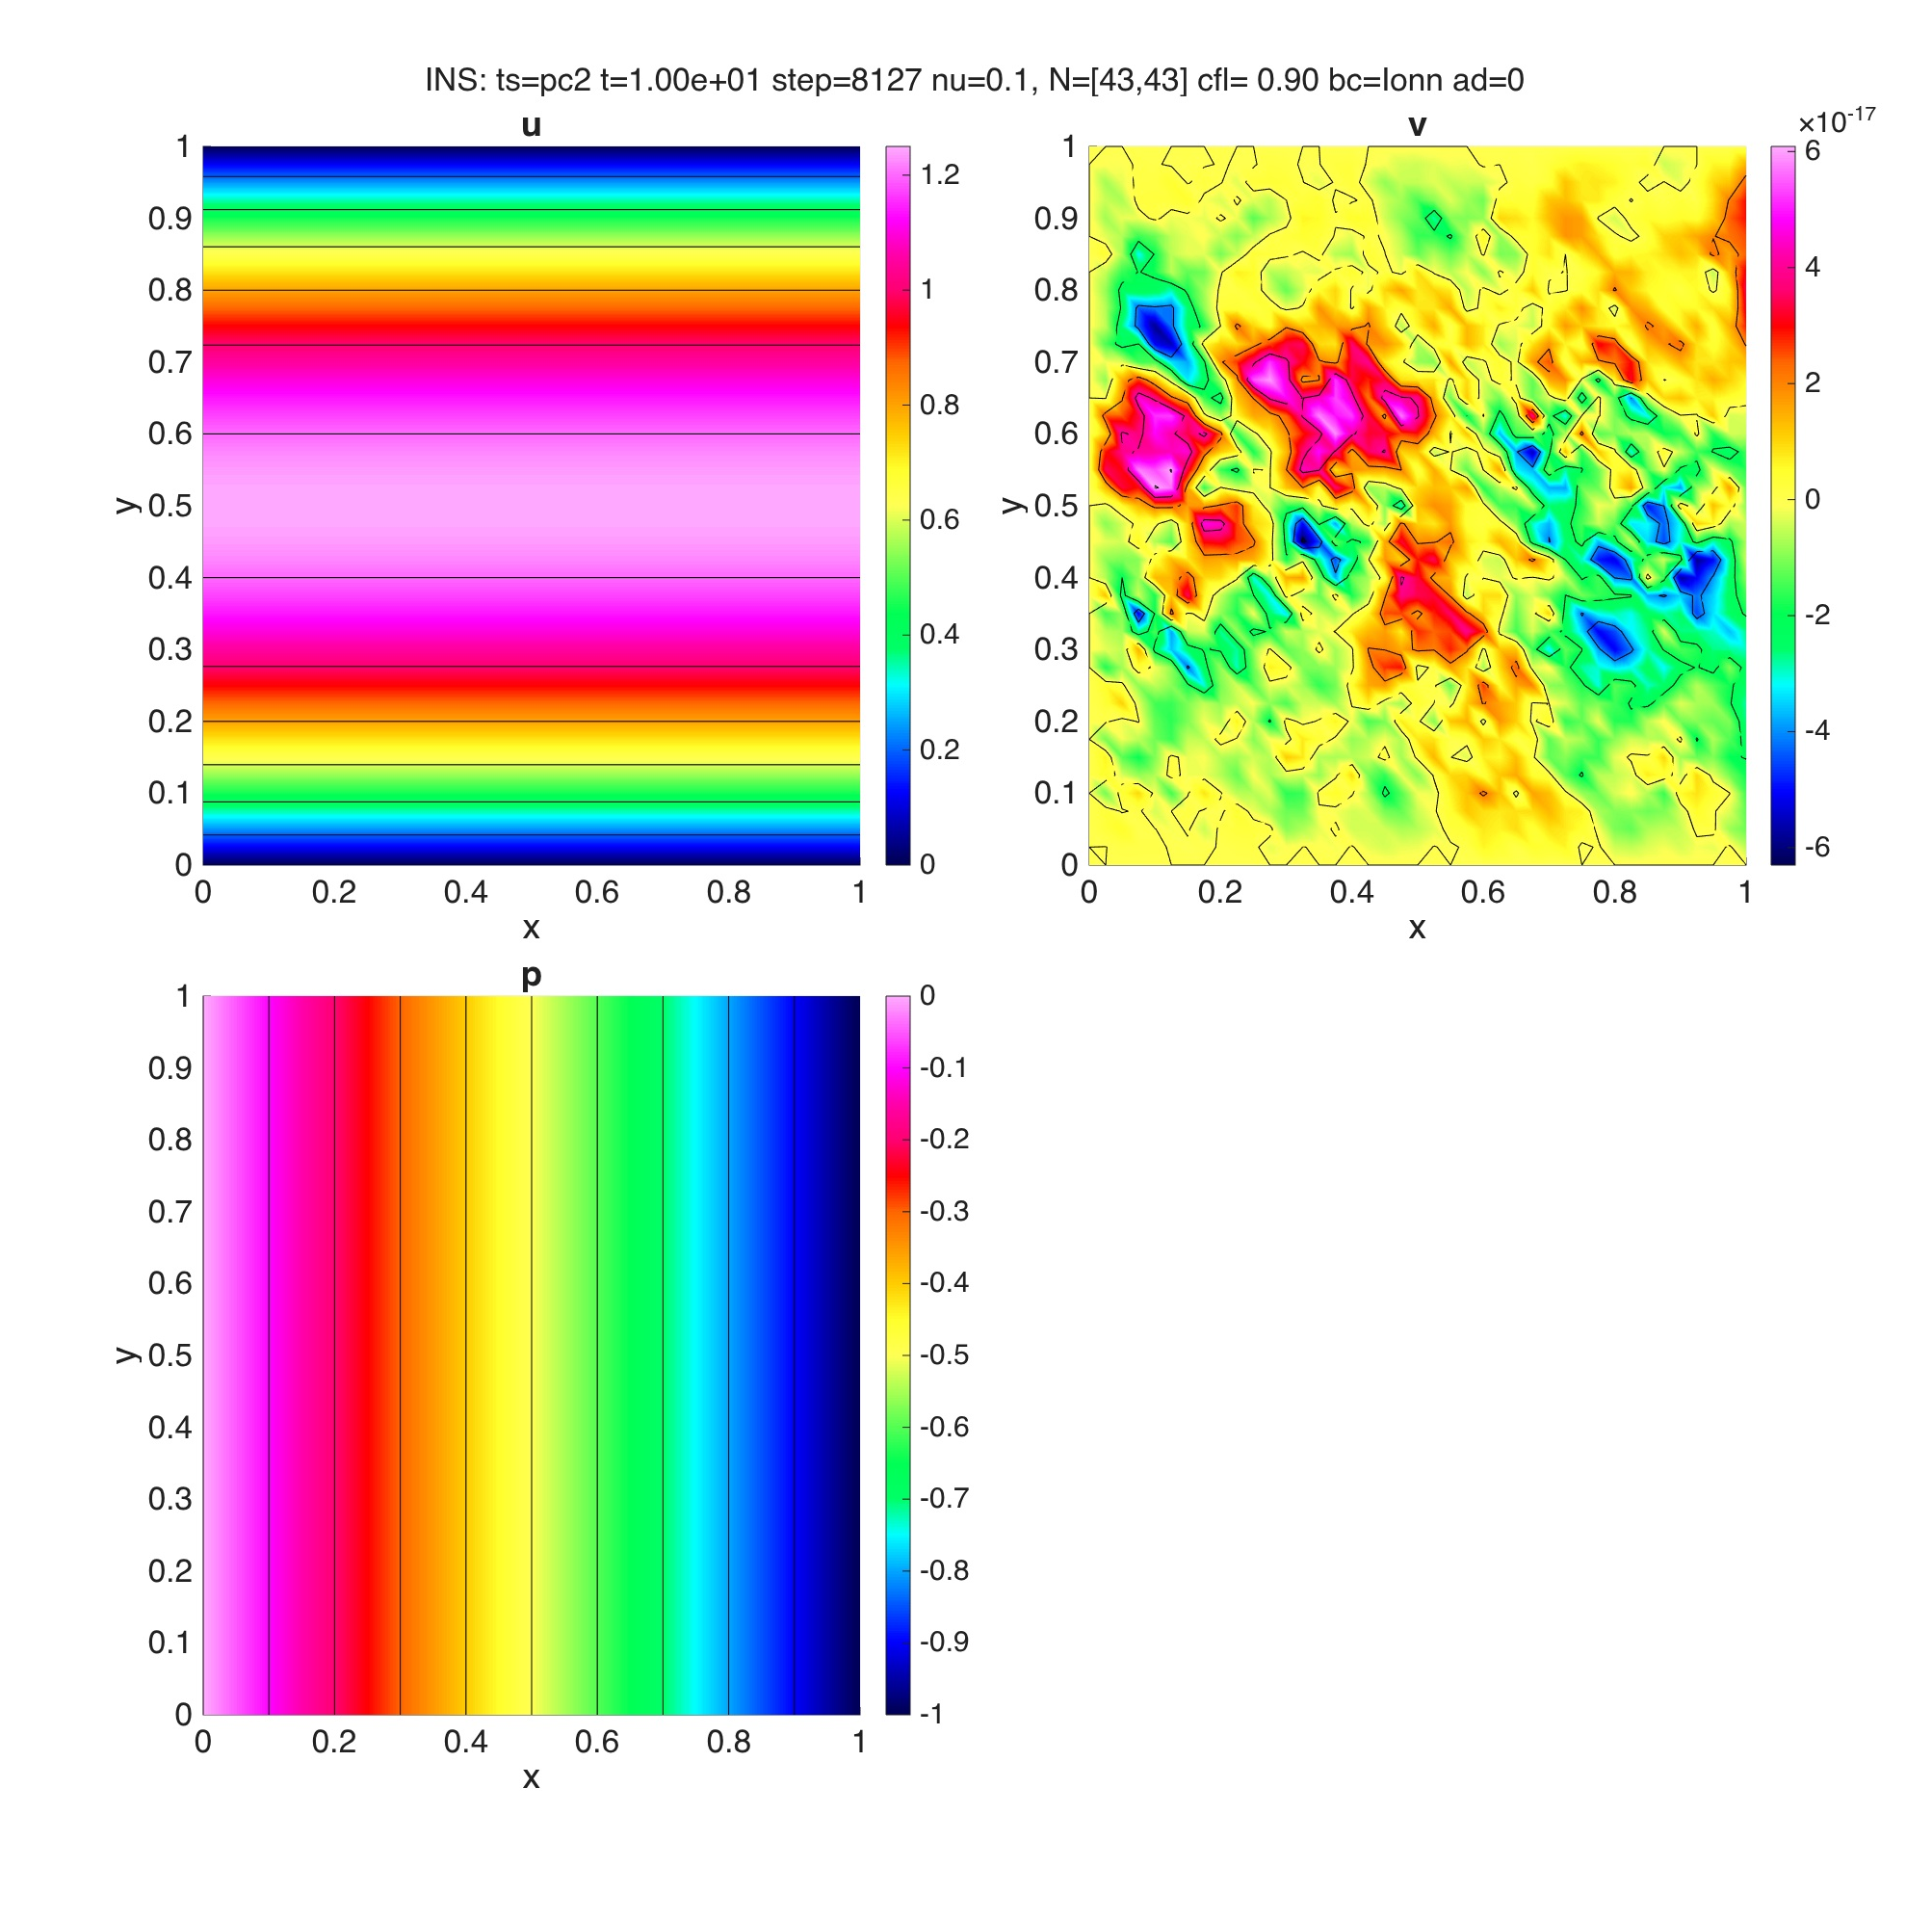
\includegraphics[width=0.8\linewidth]{../fig/PoiseuilleFlow.pdf}
\flushleft

Moreover, given the Reynolds number of the flow is not large, the plane Poiseuille flow is a stable steady-state of the INS equations, meaning if we perturb the Poiseuille flow with some other velocity profile $\mathbf u_p(x, y)$ that also satisfies the boundary conditions \eqref{eq:PoiseuilleBCs} at $t = 0$:
\begin{subequations} \label{eq:PerturbationforPoiseuille}
	\begin{align}
		u(x, y, 0) &= U(y) + \varepsilon u_p(x, y) \\
		v(x, y, 0) &= \varepsilon v_p(x, y)
	\end{align}
\end{subequations}
As our flow evolves, we should expect it to retain its form from \eqref{eq:Poiseuille} as time evolves. In the code this is tested with the following perturbation
\begin{align} \label{eq:PerturbedInitialProfile}
	u_p &= (\cos^3 (2 \pi x) + \cos(2 \pi (x + y))) \sin( 2 \pi y ) \\
	v_p &= \sin( 2 \pi x ) \sin (2 \pi y)
\end{align}
Looking at the fluid evolve over a short time scale, we can see that the fluid quickly returns to the parabolic profile as desired:
\begin{Verbatim}[fontsize=\small]
ins -ts=pc2 -tf=0.02 -N0=40 -nu=0.1  
  -ic=perturbedPoiseuille -perturbation=2.5e-1 -bcs=Ionn
  -pressureInflowValue=0 -uInflow=0 -outflowPressureCoeffp=1 -outflowPressureCoeffpn=0 -pOutflow=-1;
\end{Verbatim}
\center
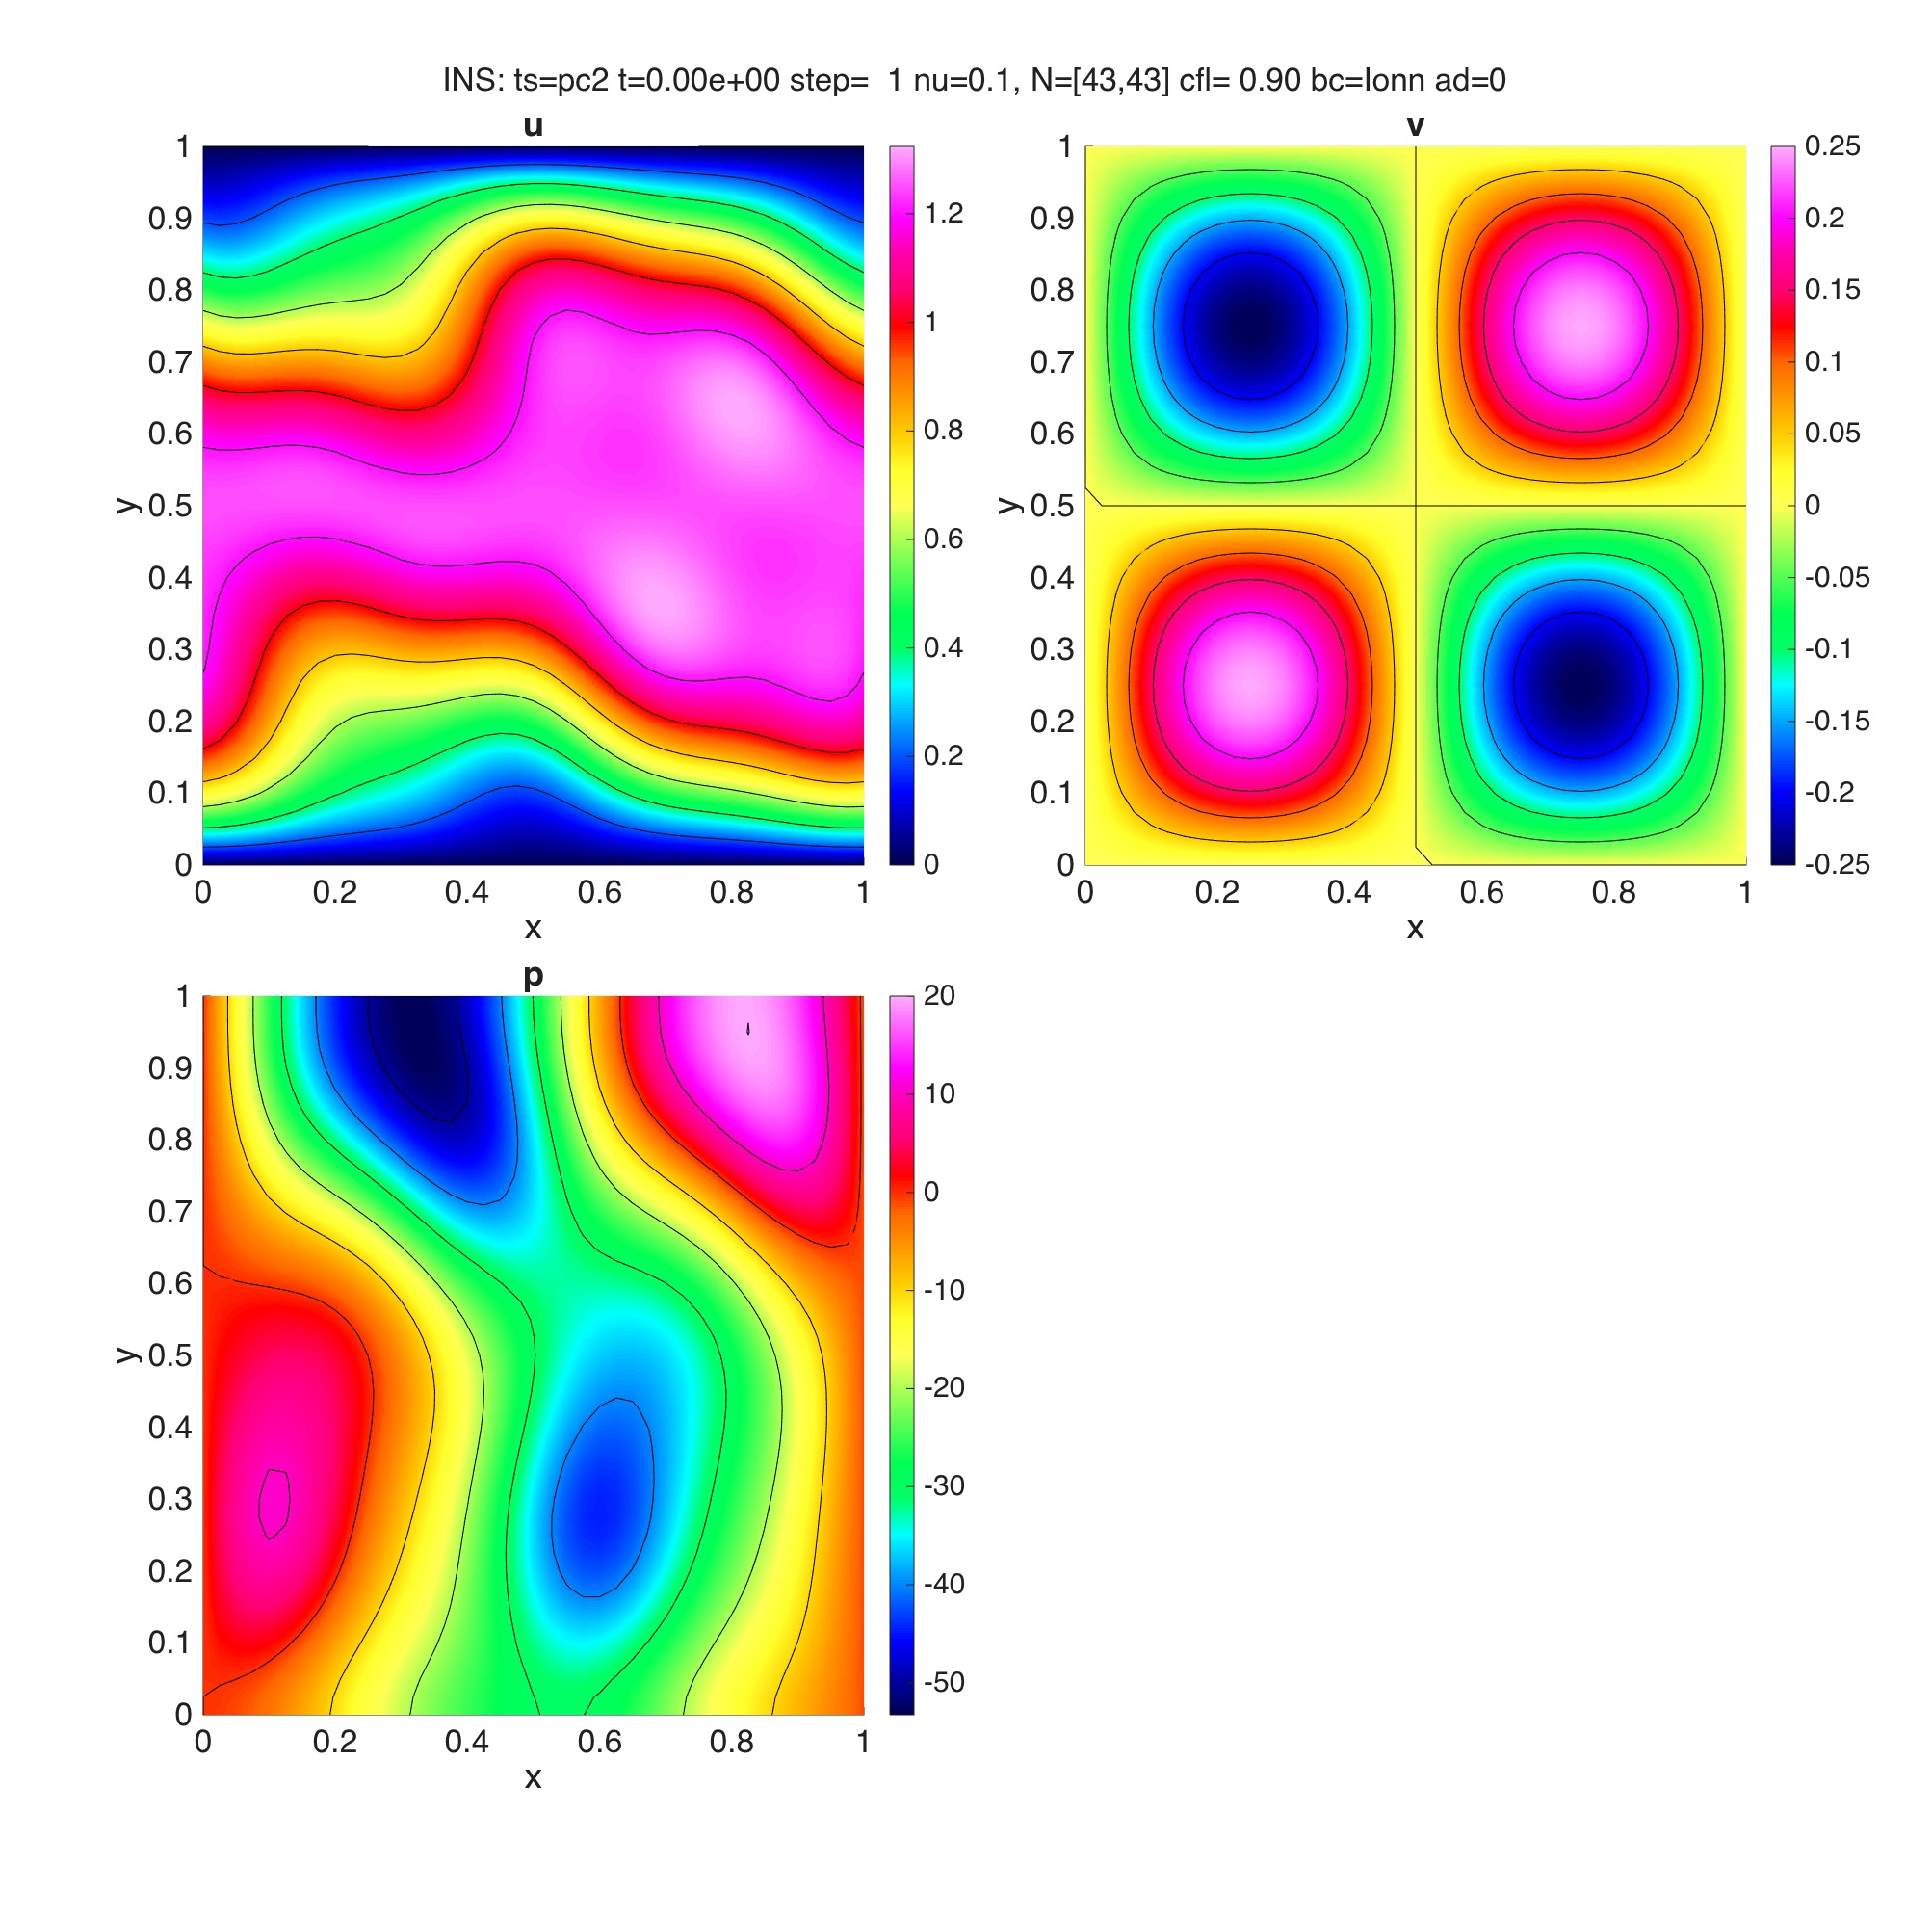
\includegraphics[width=0.8\linewidth]{../fig/PerturbedPoiseuillet0.pdf}\\
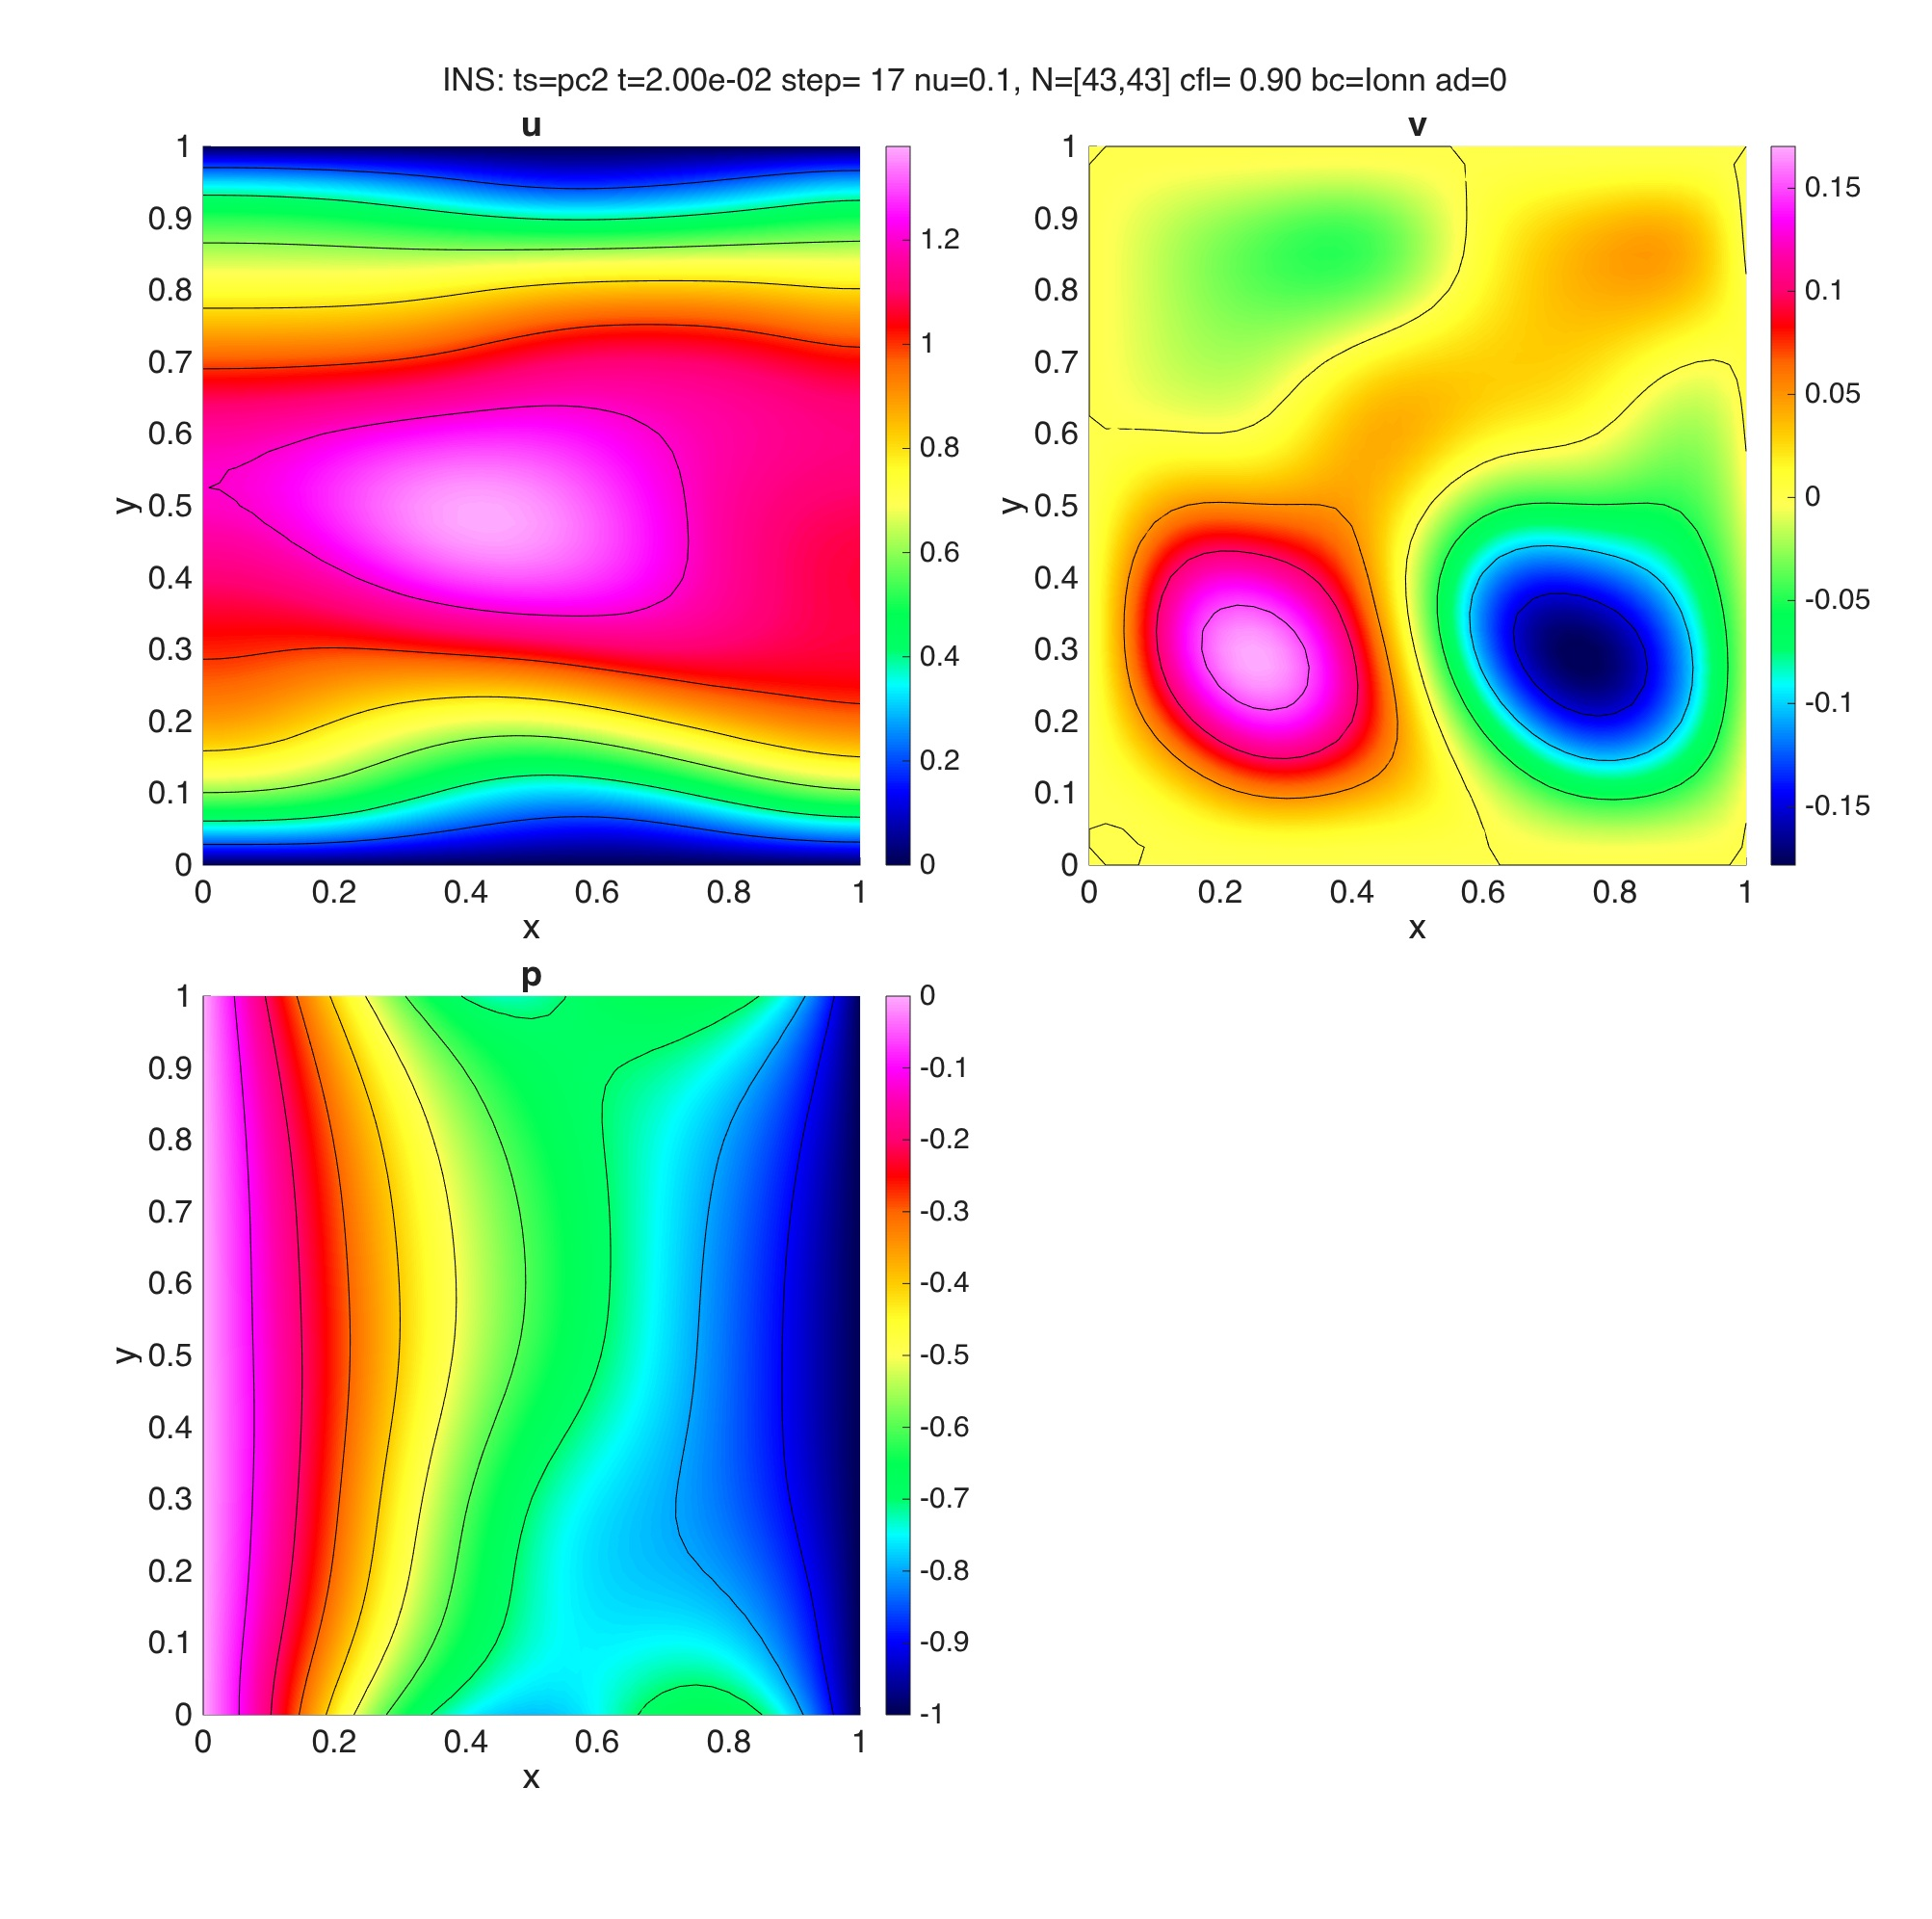
\includegraphics[width=0.8\linewidth]{../fig/PerturbedPoiseuillet2e-2.pdf}
\flushleft


% ------------------------------------------------------------------------------------
\clearpage
\subsection{Travelling Wave of a Linearized Surface} \label{sec:travelling_wave_linear_surface}
Consider an irrotational fluid flow such that there exists a scalar function $\varphi$ where
\begin{align} \label{eq:VelocityPotentialDefinition}
	\mathbf u &= \nabla \varphi
\end{align}
Then assuming that for a given wave number $k = 2 \pi n / L$ that the free surface is a travelling wave of amplitude $0 < \eta_0 \ll 1$
\begin{align} \label{eq:FreeSurface}
	\eta(x, t) &= \eta_0 \cos(kx - \omega t)
\end{align}
We have that our equation for the velocity potential and dispersion relation is given by
\begin{subequations}
\begin{align} \label{eq:FreeSurfaceEquations}
	\varphi(\mathbf x, t) &= \frac{g}{ \omega } \left( 1 + \frac{k^2L^2}{\text{Bo}} \right) \frac{ \cosh( ky + kH) }{ \cosh(kH) } \cdot - \eta_0 \sin(kx - \omega t) \\
	\omega^2 &= kg \left( 1 + \frac{k^2 L^2} {\text{Bo}}  \right) \tanh( kH )
\end{align}
\end{subequations}
And the pressure of the fluid given by

\begin{align} \label{eq:Pressure}
	p &= p_0 - \rho ( \varphi_t + g y)
\end{align}


% -------------------------------------------------------------------
\clearpage
\subsection{Taylor Green vortex} \label{sec:taylor_green_vortex}

The Taylor Green vortex is an exact solution given by
\bse
\ba
  u &=+\alpha \sin(k x) \cos(k y) F(t) \\
  v &=-\alpha \cos(k x) \sin(k y) F(t) \\
  p &= \f{\rho\alpha^2}{4} ( \cos(2 k x) + \cos(2 k y) ) \, F^2(t) \\
  F(t) &\eqdef \exp( -2 \nu k^2 t )
\ea
\ese
where $\alpha$ is a parameter defining the initial amplitude.

\mni
Figure~\ref{fig:TaylorGreenVortex} shows some results using the command
\begin{Verbatim}[fontsize=\small]
ins -ts=im2  -tf=.5 -ms=none -knownSolution=TaylorGreen -idebug=1 -nu=0.1 -bcs=nnnn -N0=100 -plotOption=1
\end{Verbatim}

{
\newcommand{\figSizeWide}{16cm}
\newcommand{\figSize}{9cm}
\newcommand{\figHeight}{4.5cm}

\begin{figure}[htb]
\begin{center}
\begin{tikzpicture}[scale=1]
  \useasboundingbox (0, 0.6) rectangle (16,9.5);  % set the bounding box (so we have less surrounding white space)


  \begin{scope}[yshift=\figHeight]
    \figByWidthb{ 0.0}{0}{../fig/insTaylorGreenVelocityAndPressure}{\figSizeWide}[0.03][0.02][0][0];
  \end{scope}  

  \begin{scope}[yshift=0cm]
    \figByWidthb{ 0.0}{0}{../fig/insTaylorGreenVorticityAndStreamLines}{\figSize}[0.05][0.01][0.05][0.05];
    % \figByWidth{ 5.0}{0}{../fig/waveHoltz1DO4TENx32Omega6BdcEMGMRESHelmholtzSolutions}{\figSize}[0][0][0][0];
    % \figByWidth{10.0}{0}{../fig/waveHoltz1DO4TENx32Omega6BdcEMGMRESMuFunction}{\figSize}[0][0][0][0];
  \end{scope}  

  % Draw grid for placing figure:
  % \draw[step=1cm,gray] (0,0) grid (16,9.5);
\end{tikzpicture}
\end{center}
\caption{Taylor Green vortex
    } 
\label{fig:TaylorGreenVortex}
\end{figure}
}



% -------------------------------------------------------------------
\clearpage
\subsection{Shear flow in a periodic channel}

Figure~\ref{fig:shearFlow} shows the roll-up of a shear flow in periodic channel.
The initial condition is perturbed shear flow
\ba
  & u(x,y,0) = \tanh( \beta ( y-y_m) ) , \\
  & v(x,y,0) = \delta\cos( 2\pi (y-y_m)) ) \sin( 2 \pi k_x x ) 
\ea
\begin{Verbatim}[fontsize=\small]
ins -ts=pc2 -tf=2.0 -tp=0.5 -ms=none -knownSolution=none -idebug=1 -nu=.0002 -ya=-.5 -yb=1.5 -xb=2
 -bcs=ppnn -N0=800 -ic=shear -movieMode=1 -plotOption=3 -plotErrors=0 -kx=1 -checkTimeStep=20 
 -ad=1 -ad21=.1 -ad22=.1 -cfl=0.95
\end{Verbatim}
Artificial dissipation is added.


{
\newcommand{\figSizeWide}{16cm}
\newcommand{\figSize}{9cm}
\newcommand{\figHeight}{4.5cm}

\begin{figure}[htb]
\begin{center}
\begin{tikzpicture}[scale=1]
  \useasboundingbox (0,.6) rectangle (16,9.5);  % set the bounding box (so we have less surrounding white space)


  \begin{scope}[yshift=\figHeight]
    \figByWidthb{ 0.0}{0}{../fig/insShearN800t2p0VelocityAndPressure}{\figSizeWide}[0.03][0.02][0][0];
  \end{scope}  

  \begin{scope}[yshift=0cm]
    \figByWidthb{ 0.0}{0}{../fig/insShearN800t2p0VorticityAndStreamLines}{\figSize}[0.05][0.01][0.05][0.05];
    % \figByWidth{ 5.0}{0}{../fig/waveHoltz1DO4TENx32Omega6BdcEMGMRESHelmholtzSolutions}{\figSize}[0][0][0][0];
    % \figByWidth{10.0}{0}{../fig/waveHoltz1DO4TENx32Omega6BdcEMGMRESMuFunction}{\figSize}[0][0][0][0];
  \end{scope}  

  % Draw grid for placing figure:
  % \draw[step=1cm,gray] (0,0) grid (16,9.5);
\end{tikzpicture}
\end{center}
\caption{Rollup of a shear flow in a channel.
    } 
\label{fig:shearFlow}
\end{figure}
}

\mni
Here are the timings on a Mac-book pro showing that most of the time is spent in solving for the pressure.
\begin{Verbatim}[fontsize=\small]
  ------------- TIMINGS pc2 Nx=800 Ny=800 Nt= 1005 --------------------
                  cpu (s)     %   
Total             5.89e+02  100.0
  setup           7.09e+01   12.0
  getUt           1.16e+02   19.7
  implicit solve  0.00e+00    0.0
  implicit factor 0.00e+00    0.0
  pressure solve  3.75e+02   63.7
  bc              3.50e-01    0.1
  plotting        2.03e+01    3.4
\end{Verbatim}
